\pagebreak
\subsection{Sequence Diagram}

\paragraph[]{Sequence diagram for traditional product entity update.} \hspace{1mm} \par
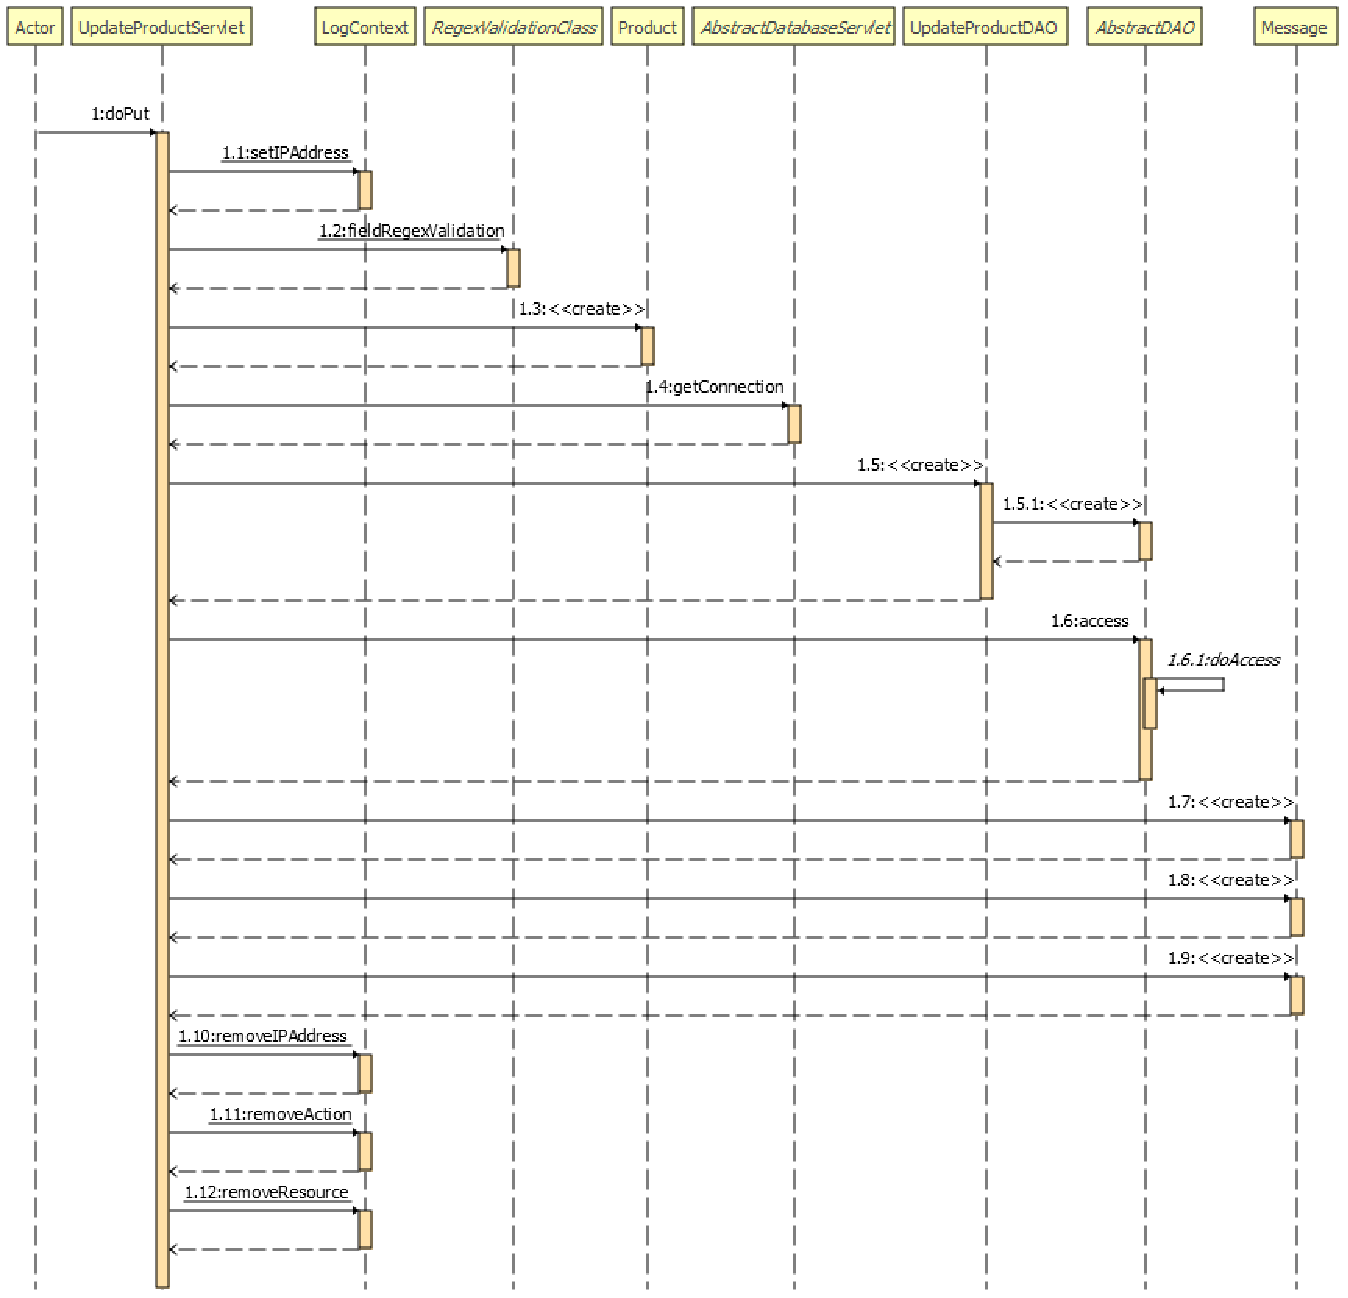
\includegraphics[width=\textwidth, keepaspectratio]{resources/updateproductsequence.pdf}
In the schema above is shown the sequence diagram for the update of a product (servlet + \textit{DAO}). 

The user sends a \textit{PUT} request to the web server. The web server calls the \textit{UpdateProductServlet} and then sets the \textit{IP} address of \textit{LogContext} and also checks, using the class \textit{regex validation}, that the parameters passed as inputs are valid.

Then a new object of class \textit{Product} is created, with the parameters passed in input. After this, the \textit{UpdateProductServlet} calls the \textit{getConection()} method of the \textit{AbstractDatabaseServlet}. After doing this, the servlet instantiate a new object of the class \textit{UpdateProductDAO}, which extends \textit{AbstractDAO}.

Then, with the \textit{doAccess()} method of the class \textit{AbstractDAO}, the \textit{DAO} connects to the database.

After connecting to the database and executing the \textit{SQL} statement, three messages for the servlet are created.

Finally, the resources are removed for the clean-up.
\pagebreak
\paragraph[]{Sequence diagram for the \textit{REST} resource \textit{``get customer''}.} \hspace{1mm} \par
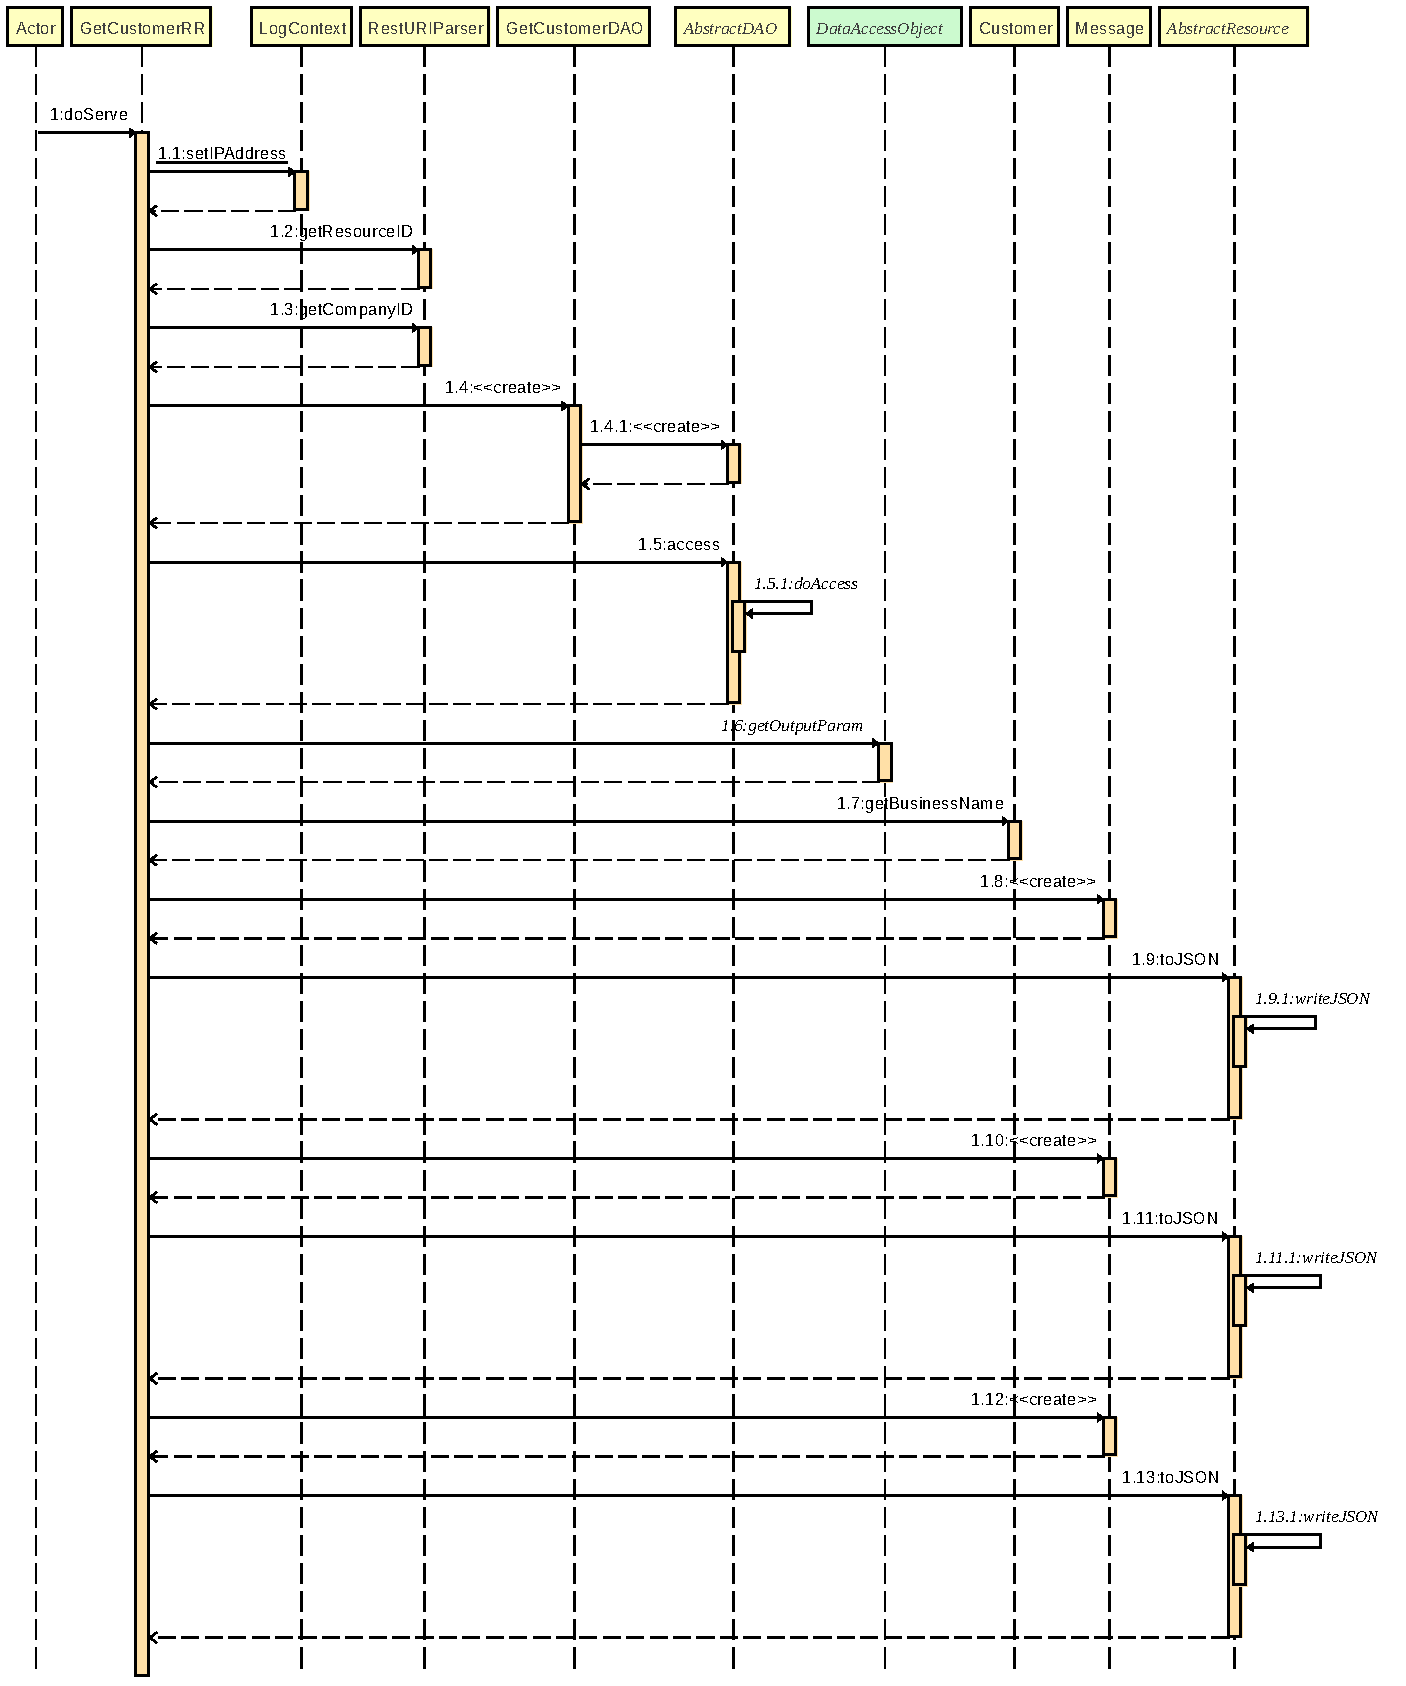
\includegraphics[width=\textwidth, keepaspectratio]{resources/getcustomersequence.pdf}
In the schema above is shown the sequence diagram for the get of a customer (rest resource + \textit{DAO}). 

The user sends a \textit{GET} request to the web server, which analyzes the request and calls the \textit{GetCustomerRR}. This class calls the \textit{setIPAddress()} of the \textit{LogContext} and then retrieves the \textit{URI} parameters with the \textit{getResourceID()} and \textit{getCopanyID()} of the \textit{RestURIParser} class.

After having the parameters stored, an instance of the class \textit{GetCustomerDAO} is created by the \textit{REST} resource, and also an instance of \textit{AbstractDAO} is created since the \textit{GetCustomerDAO} extends \textit{AbstractDAO}. The \textit{DAO} accesses the database with the \textit{doAccess()} method and retrieves the customer.

The servlet calls the \textit{getOutputParam()} method of the \textit{DataAccessObject} class and gets the output parameters asked by the user. An instance of the \textit{Customer} class is retrieved and, with the \textit{getBusinessName()} method, the servlet gets the business name of the customer retrieved.

After doing all of this, three messages are created and, with the \textit{toJSON()} method of the \textit{AbstractResopurce} class, a \textit{JSON} with the data of these messages is written (with \textit{writeJSON()}). The content of this message is based on the results of the GET request.